\documentclass[a4paper,12pt]{article}

\title{Ryder QFTゼミ資料}
\date{\today}
\author{Max Miyazaki}

\usepackage{amsmath}
\usepackage{amssymb}
\usepackage{ascmac}
\usepackage{amsfonts}
\usepackage{color}
\usepackage[dvipdfmx]{graphicx}
\usepackage{geometry}
\geometry{a4paper, margin=1in}
\usepackage{float}
\usepackage{bm}


% Define braket-like commands
\newcommand{\bra}[1]{\left\langle #1\right|}
\newcommand{\ket}[1]{\left|#1\right\rangle}
\newcommand{\braket}[2]{\left\langle #1\middle|#2\right\rangle}
\newcommand{\brakets}[3]{\left\langle #1\middle| #2 \middle|#3 \right\rangle}


\begin{document}
\maketitle
\section*{\textrm{5章 経路積分}}
\subsection*{\textrm{5.5 経路積分のさらなる特性}}

我々は、 \( q_i, t_i \) から \( q_f, t_f \) への遷移振幅が次式で与えられることを示した.

\begin{equation*}
\langle q_f, t_f | q_i, t_i \rangle = N \int \mathcal{D}q \exp \left[ \frac{i}{\hbar} \int_{t_i}^{t_f} L(q, \dot{q}) \, dt \right]
\end{equation*}

ここで \( H = \left( p^2/2m \right) + V(q) \) は現在の目的に対して十分に一般的であり, 境界条件は次のように与えられる.

\begin{equation*}
q(t_f) = q_f, \quad q(t_i) = q_i.
\end{equation*}

この種の境界条件は, 古典的な粒子の運動では適切かもしれないが, それは場の理論では用いられない. その類似物は, 例えば \( \psi(t_i) = \psi_i, \psi(t_f) = \psi_f \) である. しかし実際に起こるのは, 粒子が生成され(例えば衝突によって), それらが相互作用し, 観測によって破壊される(すなわち, 検出される)ことである. 例えば, \( \pi N \) 散乱の微分断面積 \( d\sigma/d\Omega \) を測定するとき, パイ中間子は \( NN \) 衝突によって生成され, それが検出されたときに破壊される.

生成の作用は源として表現され, 破壊の作用はシンクとして表現される. これはある意味で, 源とは言え, シンクである. 問題の境界条件は図5.6に示されるように表現される. 時間 \( t = -\infty \) で真空へと進化し, 時間 \( t = +\infty \) で再び真空へ進化する, つまり生成, 相互作用, 破壊のプロセスを通じて, 源の作用によってである. 我々は, この源の存在下での真空から真空への遷移振幅を知りたい.

\begin{figure}[H]
    \centering
    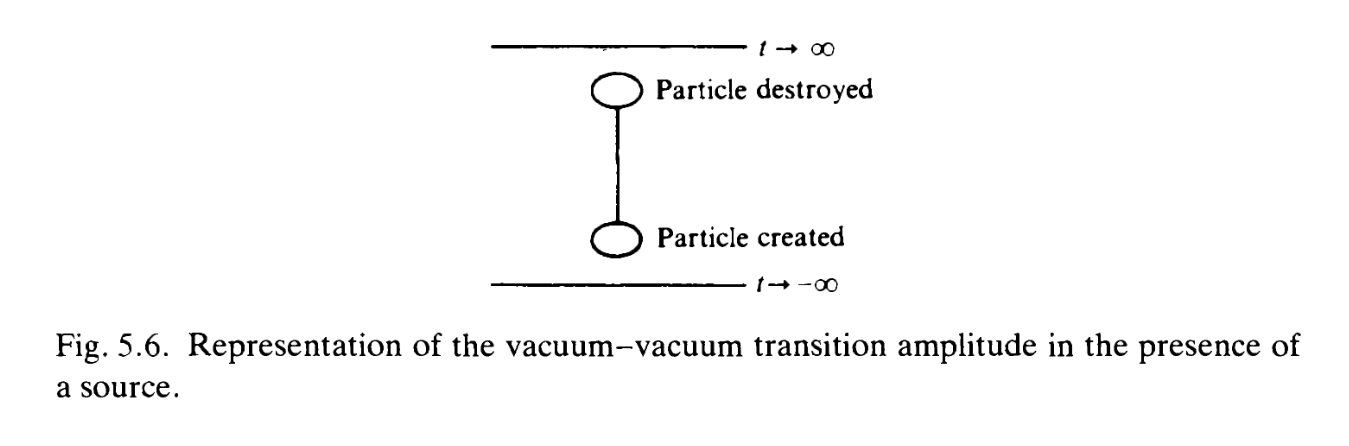
\includegraphics[width=\textwidth]{figure/fig5-6.png}    
\end{figure}

この表現は, シュウィンガー (1969年) に由来し, 源 \( J(t) \) はラグランジアンを次のように修正することによって表される. 

\begin{equation*}
L \rightarrow L + \hbar J(t)q(t). \tag{5.60}
\end{equation*}

もし \( | 0, t \rangle \) が源の存在下での基底状態(運動する基準系)で, そのときシステムが式(5.60)で記述されるとき, 遷移振幅は

\begin{equation*}
Z[J] \propto \langle 0, \infty | 0, -\infty \rangle^J \tag{5.61}
\end{equation*}

ここで比例定数は省略されている. 源 \( J(t) \) は電磁場の「源」として作用する電流と類似した役割を果たす. 荷電スカラー場 \( \phi \) は例えばラグランジアン (3.65) を持ち, それが電磁場 \( A^\mu \) と相互作用する ($A^\mu$ はラグランジアン (3.73)で与えられ, その形は $J_\mu A^\mu$). このアイデアはシュウィンガーによって一般化され, 任意の場が \( J \) によって「生成」される. \( Z[J] \) は \( J \) の汎関数であり, 我々は現在その表式を導き出す, すなわち, 基底状態への振幅は比例定数を無視して次のようになる. 本質的な特徴は基底状態の存在であり, それがどのように到達するかを説明する.

この状況は, 図5.7に示される時間軸の回転により説明される. 源 \( J(t) \) は, \( t \) と \( t' (t' < t) \) の間でゼロではなく, したがって, 遷移振幅は次のようになる.

\begin{equation*}
\langle QT' | QT \rangle^J = N \int \mathcal{D}q \exp \left[ \frac{i}{\hbar} \int_T^T d\tau (L + \hbar Jq) \right]. \tag{5.62}
\end{equation*}

\begin{figure}[H]
    \centering
    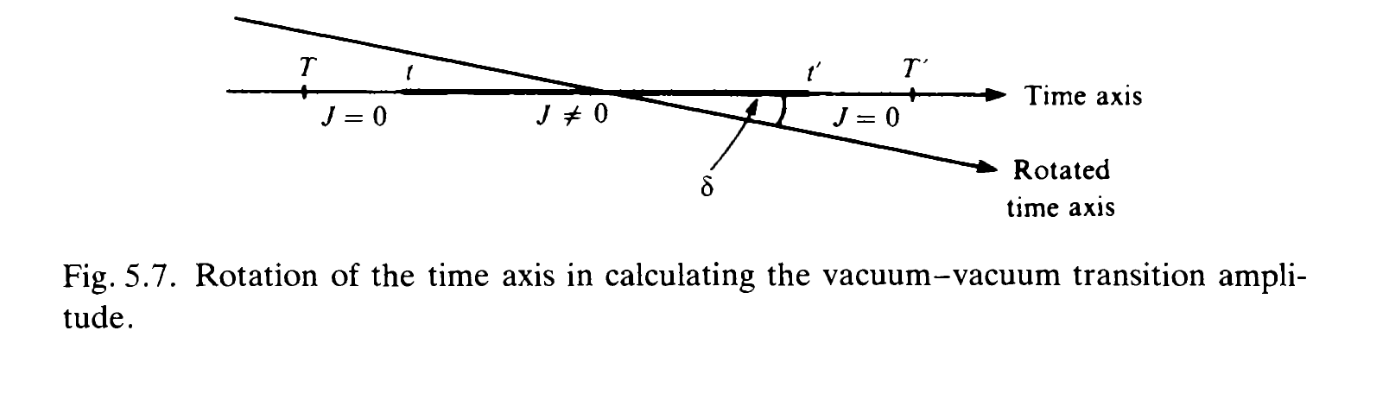
\includegraphics[width=\textwidth]{figure/fig5-7.png}    
\end{figure}

我々は

\begin{equation*}
\langle Q'T' | QT \rangle^J = \int dq' dq \langle Q'T' | q't' \rangle \langle q't' | qt \rangle \langle qt | QT \rangle. \tag{5.63}
\end{equation*}

式(5.3)を参照すると, 次のようになる.

\begin{equation*}
\langle Q'T' | q't' \rangle = \langle Q' | \exp \left( -\frac{i}{\hbar} H T' \right) \exp \left( \frac{i}{\hbar} H t' \right) | q' \rangle = \sum_{n} \phi_n (q) \phi*_n (Q) \exp\left[ \frac{i}{\hbar}E_m (t' - T') \right] \tag{5.64}
\end{equation*}

ここで, \( \phi_m(q) \) はエネルギー固有状態の完全な集合である. 同様に,

\begin{equation*}
\langle qt | QT \rangle = \sum_n \phi_n(q)\phi_n^*(Q) \exp \left( -\frac{i}{\hbar} E_n(t-T') \right). \tag{5.65}
\end{equation*}
\textcolor{red}{ここの文章結構かけてるので後で確認\\}
これらの式を式(5.63)に代入する. リミット \( T' \to \infty e^{-i\delta}, T \to -\infty e^{-i\delta} \) を取ると, 図5.7で示されるように, \( T = i|T|\sin\delta \) によって, \( \delta \) を任意の角度として表現する. このとき, \( (i/\hbar) E_n T' \) の項は実数部を持ち, \( - (1/\hbar)|T|\sin\delta \) の項は減衰因子を与えるため, \( \exp(-(1/\hbar) E_n |T|\sin\delta) \) として現れる. このとき, 和に現れる \( E_n \) が大きいほど, すべての項が減衰し, \( E_n \) が小さいほど減衰しにくくなる. 最も減衰が少ない項は, エネルギーが最も低い項, つまり基底状態, 真空である. このため, 和に残るのは基底状態(真空)の寄与だけである. これが我々が欲しい特徴である. よって次のようになる.

\begin{equation*}
\lim_{T' \to \infty e^{-i\delta}, T \to -\infty e^{-i\delta}} \langle Q'T' | QT \rangle^J = \phi*_0(Q)\phi_0(Q') \exp \left( -\frac{i}{\hbar} E_0(T'-T) \right)\times \int dq' dq \phi_0^*(q', t') \langle q't' | qt \rangle^J \phi_0(q, t).
\end{equation*}

または

\begin{equation*}
\int dq' dq \phi_0^*(q', t') \langle q' | q \rangle \phi_0(q, t) = \lim_{T' \to -\infty e^{-i\delta}, T \to -\infty e^{-i\delta}} \frac{ \langle QT' | QT \rangle^J}{{\phi*}_{0}(Q)\phi_0(Q')\exp \left( -\frac{i}{\hbar} E_0(T'-T) \right)} . \tag{5.66}
\end{equation*}

左辺は基底状態の期待値, つまり遷移振幅の期待値を示している. \( T \) と \( T' \) の時間は任意に大きくすることができるので, 左辺は $\braket{0, \infty}{0, -\infty}^J$ へと進む. 右辺の分母は, 小さい数に比例するため, 次のようになる.

\textcolor{red}{こよより以下酷いので再度確認して修正\\}

\begin{equation*}
\langle 0, 0, -\infty \rangle^J = N \int \mathcal{D}q \exp \left( \frac{i}{\hbar} \int_T^\infty d\tau \left( L + H q + J \right) \right).
\end{equation*}

これを, 次の場の理論を考慮する際に改めて扱う. その間に, 我々は次の関係を証明する. これは \( J(t) \) に関する汎関数の微分を含む関係である.


まず, \( \langle q_i, t_i | q_f, t_f \rangle \) の代わりに, \( \langle q_f, t_f | q_i, t_i \rangle \) を考え, \( q(t_n) \) は演算子であることを覚えておかなければならない. 次に式(5.6)を考え, \( t_n \) を \( t_1, \cdots, t_n \) の1つとする. このとき,

\begin{equation*}
\langle q_f | q(t_n) | q_i \rangle = \int dq_1 \dots dq_n \langle q_f | q(t_n) | q_i \rangle \langle q_{n-1} | q(t_n-1) | q_i \rangle \cdots \langle q_1 | q_i \rangle.
\end{equation*}

式

\begin{equation*}
\langle q_{n-1} | q_i \rangle = \int dq_1 dq_2 \cdots dq_{n-1} \langle q_{n-1} | q_1 \rangle
\end{equation*}

は, 式(5.13)で示された議論と類似している. よって最終的に, 次のようになる.

\begin{equation*}
\langle q_f | q(t_n) | q_i \rangle = N \int \mathcal{D}q \exp \left( \frac{i}{\hbar} \int_{T} d\tau (L + H) \right). \tag{5.69}
\end{equation*}

次に, 我々が見つけたいものを考える. つまり,

\begin{equation*}
\langle q_f | q(t_n) | q_i \rangle.
\end{equation*}

もし \( t_n > t_m \) であれば,

\begin{equation*}
\langle q_f | q(t_n) | q(t_m) | q_i \rangle = \int dq_1 \dots dq_n \langle q_f | q(t_n) | q(t_m) | q_i \rangle \cdots \langle q_1 | q_i \rangle.
\end{equation*}

最後に,

\begin{equation*}
\langle q_f | q(t_n) | q(t_2) | q_i \rangle = \int \mathcal{D}q \exp \left( \frac{i}{\hbar} \int_T^\infty d\tau (L + H) \right). \tag{5.70}
\end{equation*}




\end{document}